\documentclass[conference]{IEEEtran}
%\IEEEoverridecommandlockouts
% The preceding line is only needed to identify funding in the first footnote. If that is unneeded, please comment it out.
% \usepackage{cite}
\usepackage{amsmath,amssymb,amsfonts}
\usepackage{algorithmic}
\usepackage{graphicx}
\usepackage{textcomp}
\usepackage{xcolor}
\usepackage{caption}
\usepackage{subcaption}
\usepackage{multirow}
\usepackage{makecell}
\usepackage{subcaption}
\usepackage{cleveref}
\usepackage[backend=bibtex,
                ]{biblatex}  

\def\BibTeX{{\rm B\kern-.05em{\sc i\kern-.025em b}\kern-.08em
    T\kern-.1667em\lower.7ex\hbox{E}\kern-.125emX}}

\addbibresource{ref.bib}

\begin{document}

\title{Coherence Traffic and Store-Value Similarity Characterization for Approximate Workloads\\
%{\footnotesize \textsuperscript{*}Note: Sub-titles are not captured in Xplore and
%should not be used}
%\thanks{Identify applicable funding agency here. If none, delete this.}
}

% \author{\IEEEauthorblockN{1\textsuperscript{st} Henry Kao}
% \IEEEauthorblockA{\textit{Dept of Electrical and Comp. Engineering} \\
% \textit{University of Toronto}\\
% Toronto, Ontario \\
% h.kao@mail.utoronto.ca}
% \and
% \IEEEauthorblockN{2\textsuperscript{nd} Victor Kariofillis}
% \IEEEauthorblockA{\textit{Dept of Electrical and Comp. Engineering} \\
% \textit{University of Toronto}\\
% Toronto, Ontario \\
% vickariofillis@gmail.com}
% \and
% \IEEEauthorblockN{3\textsuperscript{rd} Pulkit Agarwal}
% \IEEEauthorblockA{\textit{Dept of Electrical and Comp. Engineering} \\
% \textit{University of Toronto}\\
% Toronto, Ontario \\
% pulkit18181@gmail.com}
% \and
% \IEEEauthorblockN{4\textsuperscript{th} Joshua San Miguel}
% \IEEEauthorblockA{\textit{Dept of Electrical and Comp. Engineering} \\
% \textit{University of Wisconsin-Madison}\\
% Madison, United States \\
% jsanmiguel@wisc.edu}
% \and
% \IEEEauthorblockN{5\textsuperscript{th} Natalie Enright Jerger}
% \IEEEauthorblockA{\textit{Dept of Electrical and Comp. Engineering} \\
% \textit{University of Toronto}\\
% Toronto, Ontario \\
% enright@ece.utoronto.ca}
% }

\maketitle

\begin{abstract}
Parallel and shared memory applications are becoming increasingly important to fully utilize the multi-core architectures present in modern computing systems. The key to improving these systems lies within the on-chip networks connecting cores and memories. Efficient communication between nodes in the network is necessary to see further performance gains; and the primary source of communication traffic emanates from cache coherence. In this paper we characterize error-tolerant multi-core workloads in terms of generated coherence traffic and store-value similarity. In our work, store-value similarity is defined as a distribution of the relative difference between a store value and the value being overwritten in the cache line. The greater the store-value similarity, the smaller the relative differences of the stored values. As many applications are intrinsically error-tolerant, for example those who's computation use floating point data, we can gain insight from the collected metrics to reduce network coherence traffic by executing on approximate/incoherent values. We also explore the domain of approximate computing and propose a novel coherence optimization, Silent Approximate Stores (SAS). In SAS, upon a store hit, if the store value is approximately equal (determined by an application define error tolerance) to the value being overwritten in the cache line, coherence requests to other nodes will not be sent. The value is stored as is maintaining the current coherence state of the line, in return mitigating further network traffic from cache misses due to coherence invalidations.
\end{abstract}



\begin{IEEEkeywords}
blah........
\end{IEEEkeywords}


\section{Introduction}

% Uni-core processor scaling over that past decade has stagnated due to increasing power consumption for marginal performance gains. Modern computing systems are seeing proliferation into multi-core and many-core processors. Parallel and shared memory applications are becoming increasingly important to fully utilize these current and upcoming architectures. However, the communication bandwidth between compute units is the main bottleneck for further boosts in performance. The key to future advancements lies within the communication infrastructure, ...

% Memory access misses private caches are either due to the cache line not being present or in the wrong coherence states. In a write-invalidate cache coherence protocol, a store operation to a local cache which misses for any reason would send invalidation requests to remote caches with the same cache line. Subsequent load or stores in the remote caches to that line would register a miss and generate corresponding coherence requests...

% A significant portion misses due to coherence related invalidation come from silent stores \cite{Lepak2002}, storing values that exactly match what is being overwitten. This suggest that there is a high degree of value locality \cite{Lipasti1996}. Existing work has examined squashing silent stores for reduce misses and improve performance \cite{Lepak2000, Lepak2002}. We however delve into the domain of approximate computing to expolit the intrinsic error-tolerance of certain applications to minimize coherence traffic with "acceptable" loss in application output quality. We do so by first introducting a novel workload characterization metric -- \textit{store-value similarity}. \textit{Store-value similarity} describes a probability distribution of the relative difference of a store value, and the value being overwritten in a memory location. It can be used to classify which applications would benefit from computing on approximate values to trade off output quality with a reduction in NoC traffic. Higher \textit{store-value similarity} corresponds to a higher probabilty of stores overwriting a memory location with values in a narrower range. Next we propose a coherence protocol optimization, Silent Approximate Stores (\textit{SAS}) tailored for error-tolerant, approximate applications to reduce coherence traffic by exploiting stores with high \textit{store-value similarity}. The protocol implements \textit{approximate stores}, where if the relative difference between a store value and what is being overwritten is within a programmer defined tolerance, the store is completed maintaining the lines current coherence state. This minimizes coherence traffic by inhibiting invalidations to remote caches which in turn reduces the amount of misses on subsequent accesses to invalidated lines.


Uni-core processor scaling over that past decade has stagnated due to increasing power consumption for marginal performance gains. Modern computing systems are seeing proliferation into multi-core and many-core processors, thus parallel and shared memory applications are becoming increasingly important to fully utilize these current and upcoming architectures. However, the communication infrastructure and bandwidth between compute units is the main bottleneck for further improvements. This infrastructure, namely the cache coherence protocol, maintains correctness of shared memory between private caches. Although the data is kept coherent throught execution of an application, it can lead to communication inefficiencies when multiple writers access the same data (true-sharing), or data that is not logically shared but resides on the same cache line (false-sharing). This causes data to be passed back and forth between nodes which inflicts additional latency, energy, and scalability issues.

As many application domains are inherently error-tolerant (e.g., machine learning, multimedia, scientific applications), we can leaverage the approximate computing domain to trade-off precise data integrity for greater performance and energy-efficiency. We propose a coherence protocol modification, Lossy Coherence, which is built on top of existing protocols to relax the correctness of shared data values within approximate applications. Lossy Coherence  introduces an approximate store instruction (\storea) to write data to the cache lines in coherence states where a conventional store would result in a miss. The \storea instructions minimize coherence transactions for true-sharing and false-sharing at a cost of making data values incoherent between caches. We show that for several approximate applications, we gain considerable energy reduction and speedup with acceptable accuracy loss for different levels of approximation.
\section{Silent Approximate Stores Protocol}

\begin{figure}[htbp]
	\centerline{\includegraphics[scale=0.4]{figures/MESI_SAS.pdf}}
	\caption{MESI SAS}
\label{fig:mesi_sas}
\end{figure}

Make a MESI coherence diagram showing how \textit{approximate stores} loop back into current state.

Explain each \textit{approx store} transitions

Maybe explain the two variants. One where you actually store the value, and one where you don't.
\section{Related Work}

Recent work \cite{Rengasamy2015} in the domain of approximate computing and cache coherence modifies a protocol to approximate on load values to minimize the effects of false sharing in approximate applications. Processor reads to invalidated cache blocks in the L1-d would supply possibly stale data to the processor instead of stalling to wait for the coherent data. While the processor executes with the potenitally stale data, the protocol concurrently services the miss through standard coherence transactions to obtain coherent data and permissions. To the best of our knowledge, our protocol is the first to tackle these combined domains using stores to leveraging the approximate value locality in error-tolerant applications. Loads on invalid lines stems from invalidations sent by remote cores requesting exlusive access to a block on a store. Instead of extending a protocol to optimize for load misses like in the prior work, we aim our efforts at the source of the problem, the stores. By implementing \storea we are not only able to reduce the amount of store misses, but also the amount of load misses due to fewer lines being invalidated. We also save energy by reducing the amount of coherence traffic and include approaches to bound the error through programmer support.  
\section{Implementation}
\begin{enumerate}
	\item gem5 syscall Ruby memory
	\item MESI Two-level cache
	\item talk about limitations of two-level since now modern procs use 3 levels.
	\item talk about increasing simulated L1 to be effectively L2 size to get more accurate results for coherence misses.
	\item Possibly talk about Silent Approximate Stores in here
\end{enumerate}

\textbf{Problem}: Successive approximate stores that have values within the error tolerance might grow unbounded and other cache lines in private caches will become very incoherent/stale. E.g., an instruction like \texttt{a += 1}.\\
\textbf{Solution 1}: Broadcast the store value every n cycles, i.e., 100000 cycles.\\
\textbf{Solution 2}: Approximation is done up the the n-th bit, i.e., the 3rd bit so approximations are bound to be plus/minus 3 from the previous value.

\section{Evaluation}

\hk{Don't read this part yet, still working on it.}

The Lossy Coherence protocol was implemented and evaluated using gem5 under full-system simulation \cite{Binkert2011}. We model a tiled CMP with each tile having one core, private L1 caches, and one slice of a shared inclusive L2. Lossy Coherence extends an existing MOESI CMP directory protocol \cite{gem5_MOESI}. The simulation setup is detailed in Table. \ref{tab:machine_config}. Cache and DRAM energy is modeled using CACTI \cite{Muralimanohar2007}. We use the same benchmarks as described in the Motivation (Table. \ref{tab:benchmarks}).

\begin{table}[!t]
\caption{Simulated Machine Configuration}
	\begin{center}
		\begin{tabular}{|l|c|}
			\hline

			\textbf{Parameter} & \textbf{Values}\\
			\hline

			Cores & \makecell[l]{8 Cores, In-order, X86, 1GHz}\\
			\hline

			L1 & \makecell[l]{Private 32kB DCache/32kB ICache, \\ 2-Way Set Assoc., 64B Block, Pseudo-LRU, 2-cycle}\\
			\hline

			L2 & \makecell[l]{Shared, 128kB per core, 8-Way Set Assoc., \\ 64B Block, Pseudo-LRU, 10-cycle}\\
			\hline

			Coherence & \makecell[l]{Lossy Protocol (underlying MOESI)}\\
			\hline

			Network & \makecell[l]{2x4 Mesh, XY Routing, \\1-cycle hop router, 1-cycle hop link,\\ 4 Directory Controllers at Mesh Corners}\\
			\hline

			DRAM & \makecell[l]{2GB, DDR3 1600MHz}\\
			\hline

		\end{tabular}
	\label{tab:machine_config}
	\end{center}
\end{table}

\begin{figure}[t]
	\centerline{\includegraphics[scale=0.4]{graphs/coherence_saving.pdf}}
	\caption{Reduction in coherence traffic for different values of $N$ normalized to the baseline ($N = 0$) protocol. Coherence traffic is catagorized as GetX, GetS, Data, and Other.}
\label{fig:coherence_traffic}
\end{figure}

We experiment with different levels of approximation in Lossy coherence using values of $N = \{2, 4, 8\}$. Figure \ref{fig:coherence_traffic} shows a breakdown of coherence traffic where $N=0$ is the baseline protocol. We get on average 2.4\%, 7.7\%, 11.1\% reduction in coherence transactions for $N = 2, 4, 8$ respectively. Benchmark linear\_regression shows significant reduction  in coherence traffic. 64.6\%  $N = 8$, because false sharing causing high numbers of coherence misses (possible cite). L1 caches see significant reduction GetX Forwarded to remote caches from the L2 (possibly give numbers). In linear\_regression significant savings come from \storea hits on coherence invalidated line (give percentage). Similarily the adi benchmark sees a significant reduction, up to 18.0\% across all values of $N$. Benchmark adi has most \storea hits on lines in the Shared state (give percentange) which reduces GetX requests to the L2 and forwarding of data from remote caches. Coherence transaction reduction does not see much improvement for higher values of $N$ because of low temporal locality when reading and modifying data.


The reduction in coherence traffic results in energy savings within the memory heiarchy (caches and DRAM) as shown in Figure. \ref{fig:energy}. Benchmarks with greater reductions in coherence traffic correlate to greater energy savings, up to 31.5\% in $N = 8$ in linear\_regression, with 93.5\% of the energy reduction coming from the just the cache heirachy. Benchmark adi on the otherhand seeing greater savings from main memory accesses (54.4\%) of the energy savings due to silent writebacks from the L2 to Main Memory. Energy savings on average 2.4\%, 7.7\%, 11.1\% for $N = {2,4,8}$ respectively.

Figure. \ref{fig:speedup} shows the speedup gained using the Lossy Coherence compared to the baseline. Similar to energy savings, linear\_regression sees greatest speedup due to reducing the effects of false sharing, up to 67.7\% in linear\_regression and 0.8\%, 4.9\%, 9.6\% for $N = {2,4,8}$ on average across all benchmarks.

Lossy Coherence maintains an accuracy 98.4\%, 97.3\% and 96.1\% for  $N = {2,4,8}$ respectively. We measure accuracy using NRMSE.





\begin{figure}[t]
	\centerline{\includegraphics[scale=0.4]{graphs/energy_saved.pdf}}
	\caption{Percent energy saved within the memory heiarchy compared to the baseline for varying $N$.}
\label{fig:energy}
\end{figure}

\begin{figure}[t]
	\centerline{\includegraphics[scale=0.4]{graphs/speedup.pdf}}
	\caption{Percent speedup for varying $N$ compared to the baseline.}
\label{fig:speedup}
\end{figure}



\begin{figure}[t]
	\centerline{\includegraphics[scale=0.4]{graphs/output_error.pdf}}
	% \caption{TODO update plot with new orcale study data. Possible include the accuracy marker in the legend if possible.}
\label{fig:error}
\end{figure}

\input{sections/conclusion}

\nocite{*}

\printbibliography


\end{document}
